\taughtsession{Lecture}{LL1 Parsers}{2024-02-23}{1400}{Jiacheng}{}

\section{Top Down Parsing: Recursive Descent Parsers}
Last lecture, we saw the \textit{Recursive Descent Parsers} which are the coded implementation of a syntax analyser. We saw that the RDP consists of a collection of subprograms, and that there is a subprogram for each non-terminal in the grammar. Many of these subprograms are recursive, hence it's name. 

\section{Left Recursion Rules}
If a grammar makes uses of left recursion, either directly or indirectly, it cannot be used directly by a recursive-descent parse. A left recursion is where the definition is defined in terms of itself, for example $A \rightarrow A \alpha$. There are two different types of Left Recursion.
\begin{itemize}
    \item \textbf{Direct Left Recursion}, where the rule can directly invokes itself without making any progress in the parse string. For example:
    \[ A \rightarrow S \beta \]
    \item \textbf{Indirect Left Recursion}, where there are multiple stages to the left recursion as seen below:
    \begin{align*}
        S & \rightarrow A \beta \\
        A & \rightarrow S
    \end{align*}
\end{itemize}
Ultimately, left recursion leads to indefinite / non-terminating recursion. However, we are able to transform a left-recursive grammar into one that is not.

\subsection{Left Recursion Removal}
For each non-terminal involved in the Left Recursion,$A$, there are two steps which have to be undertaken. 
\begin{enumerate}
    \item Group the $A$-rules as: $A \rightarrow A\alpha_1 | \ldots A \alpha_m | \beta_1 | \beta_2 | \ldots | \beta_n $
    where $A \rightarrow A \alpha_1 | \ldots | A \alpha_m$ are rules with left recursion and $A \rightarrow \beta_1 | \beta_2 | \ldots | \beta_n$ are rules without left recursion.
    \item Introduce a new non-terminal, $A'$, and replace the original rules with:
    \begin{align*}
        A & \rightarrow \beta_1 A' | \beta_2 A' | \ldots | \beta_n A'\\
        A' & \rightarrow \alpha_1 A' | \alpha_2 A' | \ldots | \alpha_m A' | \varepsilon
    \end{align*}
\end{enumerate}

\section{Top Down Parsing: LL(1) Parsers}
LL(1) Parsers are table-driven Predictive Parsers. The LL(1) stands for the what the parser does:
\begin{itemize}
    \item 1st L: left-to-right scan of input.
    \item 2nd L: leftmost derivation
    \item ``1'': means one input symbol of lookahead
\end{itemize}

A LL(1) parser utilises: a \textit{stack} to store the symbols on the right-hand side of the productions in right-to-left order so that the leftmost symbol is on top of the stack; and a \textit{parsing table} which stores the actions (ie the rules) the parser should take based on the input token and what value is on top of the stack. 

\subsection{Example}
If we consider the following grammar:
\begin{align*}
    E & \rightarrow T\ E'\\
    E' & \rightarrow +TE' | \varepsilon\\
    T & \rightarrow FT'\\
    T' & \rightarrow *FT' | \varepsilon\\
    F & \rightarrow (E) | int
\end{align*}
Here, we have non-terminal symbols $E$, $T$ and $F$ which may stand for \verb|<exp>|, \verb|<term>|, \verb|<factor>| or other structures. $E$ is our start symbol.
\begin{table}[H]
\centering
\small
{\RaggedRight
\begin{tabular}{C{0.15\textwidth} C{0.11\textwidth} C{0.11\textwidth} C{0.11\textwidth} C{0.11\textwidth} C{0.11\textwidth} C{0.11\textwidth}}
\textbf{Top of parse stack} & \textbf{int} & \textbf{+} & \textbf{*} & \textbf{(} & \textbf{)} & \textbf{\$}\\
\hline
\hline
$E$ & $E \rightarrow TE'$ & & & $E \rightarrow TE'$ & & \\
\hline
$E'$ & & $E' \rightarrow +TE'$ & & & $E' \rightarrow \varepsilon$ & $E' \rightarrow \varepsilon$\\
\hline
$T$ & $T \rightarrow FT'$ & & & $T \rightarrow FT'$ & & \\
\hline
$T'$ & & $T' \rightarrow \varepsilon$ & $T' \rightarrow ^*FT'$ & & $T' \rightarrow \varepsilon$ & $T' \rightarrow \varepsilon$\\
\hline
$F$ & $F \rightarrow \mathrm{int}$ & & & $F \rightarrow (E)$ & & \\
\hline
\end{tabular}
} % end of rr     
\caption{Parse Table}
\end{table}

\begin{minipage}{0.2\textwidth}
    \begin{figure}[H]
        \centering
        \usetikzlibrary{shapes.multipart}
        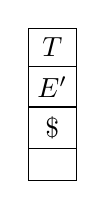
\begin{tikzpicture}[stack/.style={rectangle split, rectangle split parts=#1,draw, anchor=center}]
            \node[stack=4]  {
            \nodepart{one} $T$
            \nodepart{two}$E'$
            \nodepart{three}$\$$
            };
        \end{tikzpicture}
        \caption{Stack}
    \end{figure}
\end{minipage}\hfill
\begin{minipage}{0.75\textwidth}
    \begin{figure}[H]
        \centering
        \begin{tabular}[H]{| C{0.08\textwidth} | C{0.08\textwidth} | C{0.08\textwidth} | C{0.08\textwidth} | C{0.08\textwidth} | C{0.08\textwidth} | C{0.08\textwidth} | C{0.08\textwidth} |}
            \hline
            $($ & int & $+$ & int & $*$ & int & $\cdots$ & $\$ $\\
            \hline
        \end{tabular}
        \caption{Input Strings (tokens)}
\end{figure}
\end{minipage}

\subsection{Parsing Table}
For LL(1) parsing, the grammar is arranged into a parsing table.
\begin{itemize}
    \item The first column has the non-terminal symbols of the grammar,
    \item The first row contains the terminal symbols and $\$$ is for the end of input 
    \item The table entries give the rules of choice based on the current input (a terminal symbol) and the current non-terminal symbols (the symbol on top of the stack)
\end{itemize}

% ADD PARSING TABLE EXAMPLE

\subsection{Parsing Procedure / Algorithm}
Each step in parsing is about choosing a rule from the table according to the current non-terminal (which is on top of the stack) and current input; then pushing it's right-hand side into the stack. The $\$$ symbol represents the bottom of the stack. \\

The process begins with the start symbol ($E$ in our ongoing example). We push the right-hand side of the $E$ expression ($E \rightarrow TE'$) to into the stack, working right-to-left. This means that the top of our stack is now $T$.\\

Now, if we take the current input to be $int$. According to the table, $T \rightarrow FT'$ is selected and it's right hand side is pushed into the stack. Now the top of the stack is $F$.

% ADD TABLE
% ADD STACK EXAMPLES 